\section{Aktoren}

\subsection{Motoren}
Als einzige steuerbare Aktoren dienen uns DC-Motoren von Faulhaber mit einem integrierten Reduktionsgetriebe. Es werden 2 pro Rad zum Einsatz kommen, um ausreichend Drehmoment erzielen zu können.  Bei der ursprünglichen Variante sollten alle vier Räder je mit einem Motor angetrieben werde. Um beim finalen Design die gleiche Ausgangsleistung zu erhalten haben wir die zwei Motoren der entfernten Rädern den anderen zwei hinzugefügt.

\begin{figure}[H]
    \begin{center}
    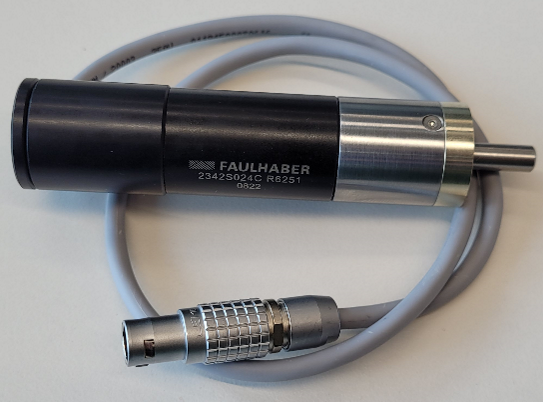
\includegraphics[width=6.3cm]{Aktoren_Motor.png}
    \end{center}
    \caption{Motor}
\end{figure}

\subsection{Peltier Element}
Das Peltier-Element in der Kühlbox erzeugt eine Temperaturdifferenz, sobald man eine Spannung daran anlegt. Mit 2 Lüftern und 2 Kühlelementen, welche in der gekauften Kühlbox bereits vorhanden sind, ist es möglich sowohl zu heizen als auch zu kühlen. \\
\\
Da die Endtemperatur von der Aussentemperatur abhängt, lässt sich hier lediglich eine Temperaturdifferenz sinnvoll definieren, welche sich auf 10-15 Grad Celsius festlegen lässt.
\begin{figure}[H]
    \begin{center}
    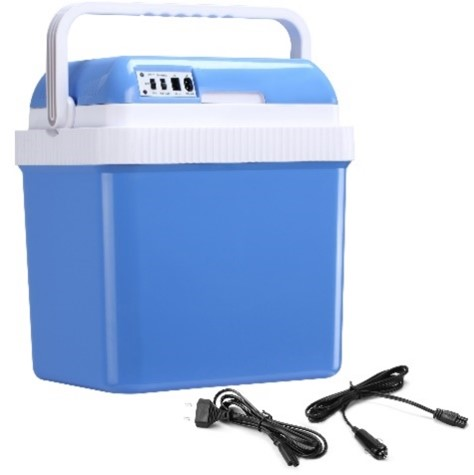
\includegraphics[width=5.5cm]{Aktoren_Peltier Element.jpg}
    \end{center}
    \caption{Kühlbox}
\end{figure}